\mycomment{\section{Tools}

Evaluating novel test representations and operations requires using
them in the context of testing real systems.  In order to facilitate
both evaluation and impact, we will be integrating our efforts with
existing tools that manipulate tests.  In a sense these tools are our
most critical preliminary work:  public, usable (and used) platforms
for making test operations available, and evaluating their utility.


\subsection{TSTL: the Template Scripting Testing Language}

TSTL \cite{tstl,NFM15,ISSTA15,tstlsttt} (the Template Scripting Testing Language) is a
Python-based domain-specific language for building test interfaces to
software systems.  TSTL has already been used to
discover faults in the widely used ArcPy GIS library \cite{ArcPy}, the
gmpy2 \cite{gmpy2,gmpy2bugs}
interface to GNU GMP \cite{gmp}, the {\tt sortedcontainers} library, the core CPython bignum
implementation \cite{cpythonbug}, PyOpenCL \cite{PyOpenCL} (or in GPU
hardware or OpenCL \cite{OpenCL} itself), the FuzzyWuzzy string
matching package \cite{FuzzyWuzzy}, the AstroPy library
\cite{AstroPy}, {\tt pyfakefs} \cite{pyfakefs}, Apple's OS X operating
system, and the
SymPy \cite{sympy} symbolic math package \cite{tstlsttt}.  TSTL represents tests as
sequences of actions, where each action consists of:  a guard
(conditions under which that action is legal ---  defining guards on
actions helps maintain validity during test operations, by
automatically disabling invalid actions) and an actual action (arbitrary Python
code, which is statically linked to the fixed set of test variables it
modifies).  Enhancing TSTL is a simple way to enable evaluation of our
methods and allows us to provide continuous release and technology
transfer, in that users of TSTL will have access to any new
operations.  TSTL already includes a powerful normalization method
\cite{OneTest} and a suite of tools for test manipulation to build on \cite{suiteunderstanding}.

\subsection{C-Reduce}

C-Reduce\cite{CReduce} takes large C or C++ files and makes them
smaller, while preserving a criterion of interest.
%
At first glance the job is simple: why not just remove lines of code,
functions, subexpressions, and other syntactical elements?
%
Of course these things need to be done, but the resulting test cases
end up being far from minimal.
%
To do a really good job at its stated goal, C-Reduce incorporates many
transformations that resemble compiler optimization passes; these do
things like inlining a function, removing a level of indirection from
a pointer, and instantiating a template.
%
All of these things require coordinated changes across many parts of a
program: no simple syntactical change will accomplish the goal.
%
In the end we wrote well over 30,000 lines of code to perform
sophisticated program manipulations.


C-Reduce is structured as a fixpoint iteration that calls
transformation passes that each implement a simple API\@.
%
It runs these passes to fixpoint.
%
When given a large input (preprocessed C++ files tend to be well over
a megabyte) this process can be slow, so C-Reduce runs its search
algorithm in parallel on a multicore machine.
%
C-Reduce is widely used in practice and it produces much smaller final
outputs than any other reducer for C and C++ that we are aware of.
%
C-Reduce's modular structure will make it an ideal piece of
infrastructure on which to do our test manipulation work.
}

\section{Research Focus 1: Test Composition for Heterogeneous Systems}

Modern critical software systems are often composed of a complex
interacting set of layers.  For example,
cyber-physical systems (CPS) design employs layering in multiple
domains, e.g., computation, networking, and the modeling of the
embedding physical system and the system's sensors and
actuators. However, current layering approaches do not capture
non-functional system properties essential to CPS, e.g., timing and
energy use, that emerge via testing.  To manage design process
complexity, iterative development is commonplace: while the long-term
trend is refinement of abstract models, engineers often need to shift
back and forth  between implementation-level models and more abstract
models to gather new data, gain knowledge and insight, and optimize
system performance.  

The same multiplicity of heterogeneous layers also often applies to existing tests
for complex systems: often components of a system,
such as a file system or actuators, are tested by one set of
engineers, and using completely different methods than are used to
produce tests at the high level of either control software with
humans-in-the-loop or autonomous control systems.  The core
functionality of a system is usually written in low-level, embedded
systems languages, such as C.  In the ideal case, such systems are
developed using both formal specification and verification and
sophisticated automated testing.  In some cases the formal
specification is used to generate executable tests to ensure the real
system matches the formal models; in other cases there is at least a
very determined test generation effort, including efforts to produce
very high-coverage tests.  In contrast, user-centric or high-level
autonomy layers are often developed in higher-level
languages, such as Java, and with a much more informal approach to
testing and verification.  Increasingly, mission- and safety-critical
low-level elements interact with users or high-level autonomy.  Even when the behavior of each system, in
isolation, is valid, the composition may compromise performance,
user experience, security and privacy, or (in the worst case) safety.

\mycomment{We propose a partial solution to this problem: automatically
\emph{composing tests}, including heterogeneous tests targeting
different layers of a system.  Often there exist tests for behaviors
at different levels, and these have considerable value --- but the
combined behaviors are not well tested, and the tests cannot be
combined.   As an example of the practical aims in this focus, it would
be helpful to run the low-level tests in one domain in the context of
other domains expressed using high-level models. For example, consider
the following closed-loop scenario: a unit-level test of
implementation-level code running on a target sensor/actuator (S/A)
node connected to a model running in the cloud that
drives an emulated transducer at the S/A node, and, through a
packet-layer communication link model, to a high-level control system
model running in real-time on an engineer's workstation; this model in
turn drives an S/A node actuator via commands sent through the
communication link model. \mycomment{As another example, existing
production-level, server-based control code may need to be integrated
with a new actuating subsystem. Here, functional tests could be
performed using a sequence of models (of increasing refinement) prior
to integration of the target actuating hardware.}  In our
running example below, even the ``same'' component of a CPS may
have multiple levels: consider the case of a file system on a
robot exploring another planet, which has both a
NAND flash file system and a high-level interface to it commanded by
humans.  While the problem of composing tests across system layers is
not unique to CPS or embedded systems, their tendency to combine
human-facing interfaces with critical components that are more
thoroughly tested makes them a primary target for such efforts.}

Existing tests for different layers are highly valuable;
however, they typically fail to cover the interaction of components
effectively.  This problem is made worse by a fundamental limitation:
tests do not compose.  Even within a single system, executing test
{\tt A}
followed by test {\tt B} seldom produces the desired union of behaviors
(e.g., even covering all code covered by {\tt A} or {\tt B}).  The
actions of {\tt A}
often interfere with those of {\tt B} (or vice versa): that is, some action
in {\tt A} is either illegal in a composed context, causing {\tt B} (and thus the
entire test) to become invalid, or
disables some behavior of {\tt B}, lowering test effectiveness.  The
ordering of test operations also matters: e.g., some actions in {\tt A} must be
before some actions in {\tt B} to produce interaction, while other actions
must be after some {\tt B} action.  For compositions of safety-critical and
user-centric systems, and heterogeneous systems in general, it would
be highly desirable to be able to automatically produce tests that are
valid, have as little interference as possible, and maximize the sum
of behaviors from the composed tests. \mycomment{ The inability to compose tests
results in poorer testing, and thus more fault-prone and brittle
systems.}  In order to achieve this goal, we propose a novel operation
of \emph{test composition}, using the existing operation of
test minimization \cite{DD,icst2014,OneTest} to remove portions of a
constructed \emph{hypothesis composition} to produce a test that has more
behavior than a na\"ive composition \cite{tecpscompose}.

\subsection{Motivating Example: Mars Rover File System Testing}

As an example of the problem, consider the following situation, a
simplified generalization of testing efforts performed by PI Groce and
others at NASA's Jet Propulsion Laboratory, during the development of
the Curiosity Mars Rover (Mars Science Laboratory project)
\cite{CFV08,ICSEDiff,AMAI}.  The file system for the rover can be
considered from two points of view.  There is the low-level, embedded
flash file system, implemented as (essentially) a library in C.  There
is also a higher-level file catalog process, through which other
components of the Curiosity software interact with the file system,
and which is directly accessed by ground operations teams.  The
low-level file system was extensively tested using both model checking
and random testing, by a team of formal verification and software
engineering researchers.  The high-level catalog process was also
tested extensively --- but only manually, by systems engineers and the
Curiosity QA team, using less formal and intensive approaches.  Every
catalog test also tests the underlying file system, of course, but
file system tests do not test the catalog.  In practice, the two sets
of tests exist completely separately: the catalog tests as Python
scripts to issue commands, and the file-system tests as C programs.
In operation, some faults related to interaction of the catalog and
the file system were discovered.  \textbf{We hypothesize that being able to
compose high-level catalog tests and low-level file system tests might
have detected some of these faults.}

Na\"ive composition of tests for the file
system and the catalog will not work.  Low-level file system tests may
include operations that change the file system state in a way that the
catalog, which has sole control of the contents of the file system in
most directories during normal rover operation, cannot handle.
Consider the composition of test {\tt A}, for the file system, and
test {\tt B} for the catalog.  Neither {\tt A+B} (composition with
{\tt A} followed by {\tt B}) nor {\tt B+A} will provide the desired
testing functionality.  If we execute {\tt A} then {\tt B}, there may be little
interaction between systems, and {\tt A} may produce an initial state
that the catalog cannot handle.  If we execute {\tt B} then {\tt A},
the much more extensive testing of the underlying flash file system
provided by {\tt A} will not impact the catalog behavior at all, resulting
in even less interaction.  How to interleave the behaviors, while
avoiding actions in {\tt A} that violate catalog constraints, is a challenge
even for engineers well-versed in both systems.  We therefore
construct a new test, {\tt (A+B)}$\times k$, consisting of {\tt A}
followed by {\tt B}, repeated $k$ times.  This test will also, due to
interference (let us assume {\tt A} violates a catalog constraint) tend to
fail immediately without exposing a real fault. How can we avoid these problems?


Test case reduction \cite{DD} works due to the high probability that contiguous parts
of a test are related: removing \emph{chunks} of a test can
eliminate many behaviors that are irrelevant or interfering.  Given
a test {\tt a1.a2.a3.a4.a5.a6.a7.a8} that fails, delta-debugging 
might first determine if
either of {\tt a1.a2.a3.a4} or {\tt a5.a6.a7.a8} fails; if so, it
proceeds from either.  If not, it increases the granularity of
reduction, and considers additional candidates, until no single
component can be
removed without the test no longer failing.  

Cause reduction \cite{icst2014,stvrcausereduce} extends
delta-debugging and other minimization approaches to reduce tests with
respect to an arbitrary property, not just failure.  For example to produce very fast
regression tests (called ``quick tests''), automated tests can be
minimized to find smaller tests that retain full code coverage.  \mycomment{In
past work, this approach produced highly efficient tests for
real-world systems such as Mozilla's SpiderMonkey JavaScript engine
and the YAFFS2 flash file system used in Android.}  
Cause reduction traditionally requires as
input a test that satisfies the property of interest, e.g., a failing
test or one with certain coverage.  However, our concept of tests
implies this is not necessary.
Given a test that does not fail (or provide some other useful property), cause reduction defines a search, based on
removal of components, for a test that \emph{does} meet the criteria.  We
first construct hypothesis compositions of tests (that do not provide
useful testing), and then use cause reduction to search for a test that \emph{does}
provide useful composition of the tests.  The search has a potential
to succeed because in most cases the reason composition fails is
interference, which can be avoided by removing the interfering parts
of a test, leaving a good interleaving of test actions, made possible
by the $k$ repetitions in the hypothesis composition.

A concrete application of our approach to the NASA Mars rover file
system testing would work as follows.  First, construct the test {\tt
  (A+B)}$\times k$.  If $k$ is at least one more than the
max of the lengths of {\tt A} and {\tt B}, then there is a possibility
(though not a guarantee) for cause reduction to produce \emph{any} needed
interleaving of actions: removing all but the needed actions from each
copy yields all interleavings of a single copy of {\tt A} and {\tt B}.
The extra copy is required so that the interleaving can start with
either of {\tt A} or {\tt B}.  We search
for a reduction of {\tt (A+B)}$\times k$ that: 1) does not violate catalog invariants, so is a valid
test, since a core problem of composition is the creation of invalid
tests and 2) covers at least the union of code
coverage for test {\tt A} and test {\tt B}, and maximizes additional
coverage due to interaction.  \mycomment{Alternatively, the search
can be for a test that fails for any reason other than catalog
invariant violation.  However, in some cases, both of these searches
may fail.}

\begin{figure}
\centering
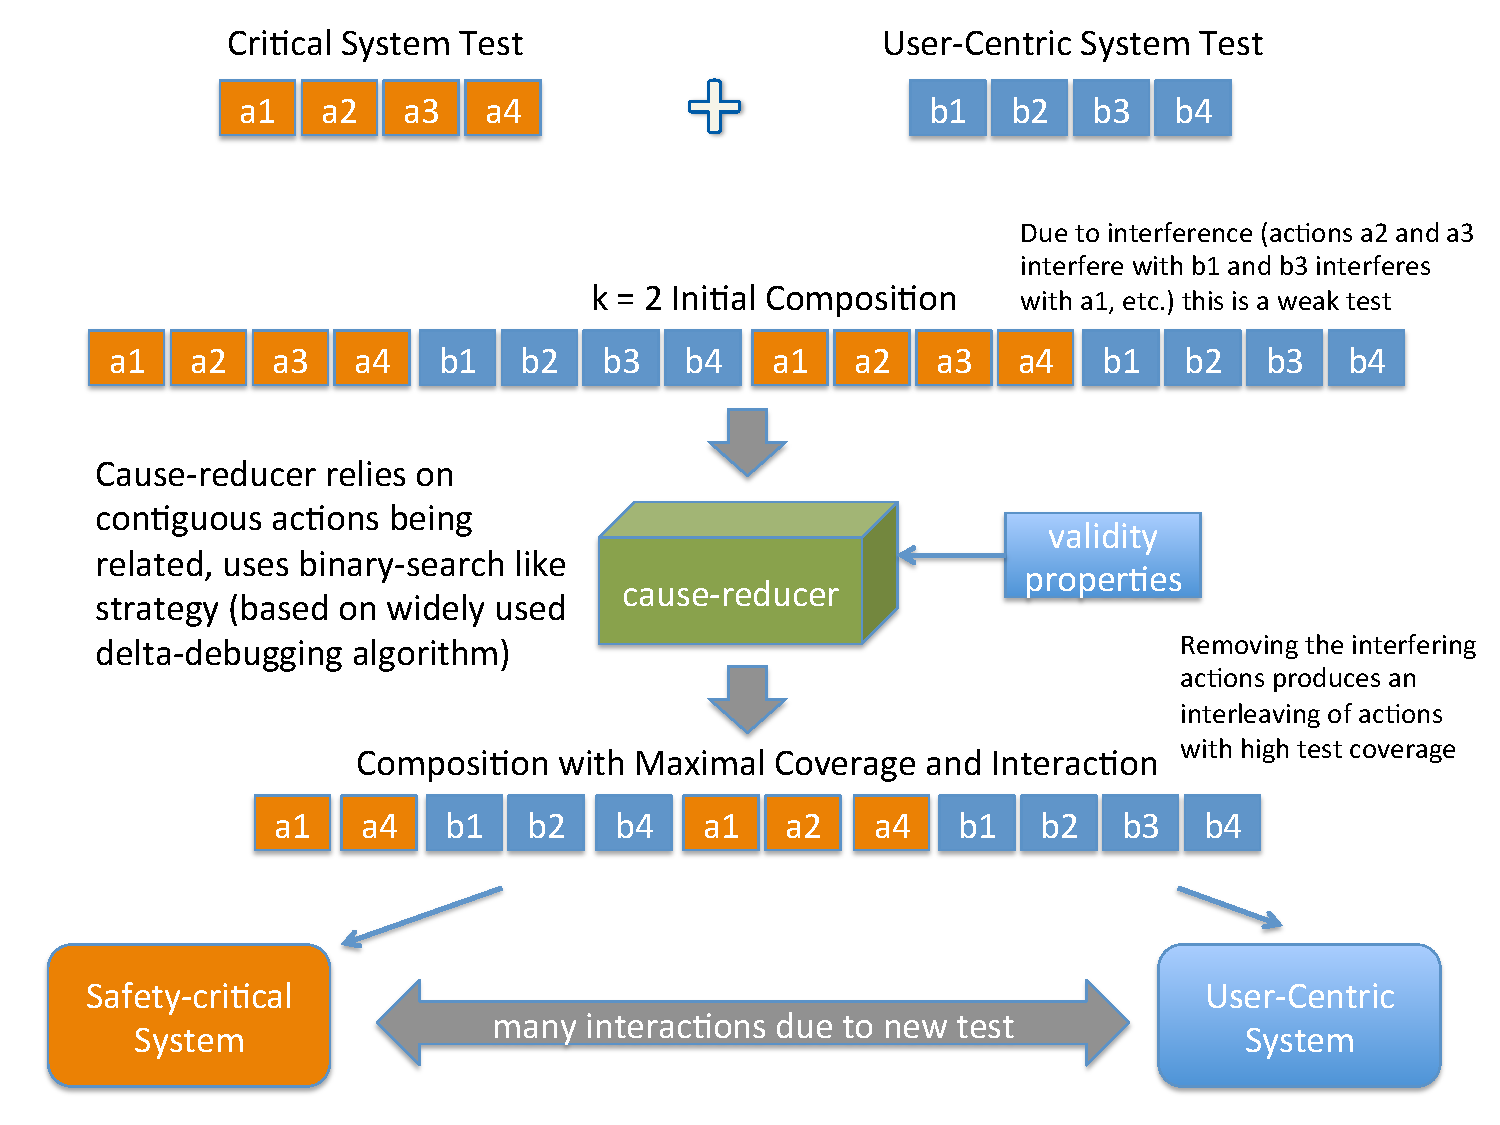
\includegraphics[width=0.6\columnwidth]{testcomp}
\caption{Composition of heterogeneous system test cases.}
\label{fig:compose}
\end{figure}


To understand the concept, consider the simple case where {\tt A =
  a1.a2.a3.a4 and B = b1.b2.b3.b4}, with $k = 3$.  If {\tt a1}
interferes with {\tt B}, causing the catalog to fail with an invariant
violated at action {\tt b3}, then our approach can produce a test such
as: {\tt a2.a3.a4.b1.b2.b3.a1.a2.a3.a4.b1.b2.b3.b4.a1.a2.a3. a4}. Here,
{\tt a1} is removed from the copy of {\tt A} before any {\tt b3}, but
remains in the final version, from which all {\tt B} actions are
removed, because it adds new code coverage of the low-level file
system.  One {\tt b4} instance is removed, because it causes the
low-level file system code to be in a state such that the second copy
of {\tt B} exercises less code (it forces an early garbage collection
of flash blocks).  Using gains in coverage to change the base test (a
variation of cause reduction we refer to as ``amplification''), we can direct
the reduction toward this high-coverage, valid, composed test without
human intervention.  Figure \ref{fig:compose} graphically shows the workflow of
automated test case composition for a different set of tests.

\subsection{Initial Results and Research Problems}

We implemented a simple version of our approach in the TSTL tool for
Python testing \cite{tstlsttt,NFM15}, and applied
it to compose tests for the {\tt pyfakefs} file system \cite{pyfakefs}.  We generated a
large set of tests containing only file operations and a large set of
tests containing only directory operations, and then applied both a
n\"aive composition approach and a simple version of our approach
(without amplification), with increasing $k$.  Directory-only tests
had a mean branch coverage of 343.3 branches, and file-only tests had
a mean branch coverage of 612.03 branches.  N\"aive composition
improved this to 651.87 mean branches, but $k=2, 3, 4$ composition improved
the means to 693.23, 698.3 and 714.37 mean branches, respectively.
All results were statistically significant, and at $k=4$, produced
tests were highly complex and using chunks of original tests as
``components'' of complex file system operations not present in either
set of simpler tests.

Because this approach suggests that test composition is essentially a
search problem, an obvious question is why we use cause
reduction/delta-debugging rather than a more traditional search-based
evolutionary or genetic algorithm approach \cite{searchtest,McMinn04search-basedsoftware,FA11}.  First, we believe that
removal of operations is the only mutation of interest in this
context: crossover or random change in test actions is likely to
introduce invalid test behavior.  Our assumption is that tests to be
composed are valid in isolation, and only nearby behaviors are of
interest (or likely to maintain single-component validity).  Second,
many search-based techniques expect access to branch distances and
other intrusive instrumentation.  This may not be feasible for
embedded systems; we can use cause reduction with instrumentation only
for user-centric code or, in the worst case, for neither system.  This
necessitates guidance by other means.


The sketch of a composition approach here is, of course, highly
incomplete. We must determine, for example, how best to choose initial
values for $k$, how to identify and make modifications to
delta-debugging that speed termination of the search or allow for
better parallelization \cite{PracMin}, and how to devise heuristics for abandoning a
failing search and using a larger $k$.  Other basic research questions
are numerous: e.g., is it best to first amplify for coverage, then
search for faults, or is this inefficient?

As an example of the kind of research question each new operation for
tests introduces, consider the fact that for some systems composition
of more than two tests may be essential to exploring interactions.
However, composing more than 4-5 tests may make cause reduction
prohibitively expensive.  How to choose only tests likely to yield
critical interactions is a novel and interesting test selection
\cite{YooHarman} problem; does composition compose?  That is, for
truly first-class tests we would expect that {\tt (A+B) + (C+D) =
  A+B+C+D} but this is far from clear in the context of test
composition, where {\tt C} and {\tt B} may have unavoidable
interference.  Another key research issue is how to extend the number
of cases where composition can succeed.  In some cases, composition of
two tests cannot proceed without ``bridging'' actions contained in
neither test.  Some bridging actions may be possible to generate
automatically, through static analysis of tests (variable renamings,
object creation and deletion, etc.), or via the same term rewriting
approach taken in normalization.  Others may require generating
random actions \cite{HamletOnly,RandFormal,DirectedSwarm,Pacheco} that cause reduction can discard if they are not needed
or are interfering.  We expect that other complexities will arise
during experimentation.

We plan to use test composition as an initial benchmark operation to
refine our ideas of tests as first-class entities, and the building
blocks required to build complex operations over tests in general
settings.

\section{Research Focus 2: Test Composition for Compilers}

Although widely-used compilers such as GCC and LLVM typically work
well in the common case, many bugs lurk in dark corners of C and C++
that are exercised by relatively few programs, and where the
standards shed little light.
%
It also tends to be very easy to trigger compiler bugs when using
esoteric compiler options and when targeting new or little-used
chipsets.


GCC and LLVM each come with thousands of unit tests that are somewhat
effective at preventing new bugs from being introduced into the code
base.
%
These compilers, which we have extensive experience
testing\cite{csmith}, will be ideal testbeds for first class
test operations.
%
The issue of validity (freedom from undefined behavior) is particularly tricky
for test cases in C and C++\cite{EllisonRosu12POPL}, in contrast to
the simple guard-based approach of TSTL.
%
Validity is undecidable in principle and difficult to
establish in practice --- as evidenced by the difficulty that the
computing community has had in eliminating undefined behaviors in
Internet-facing software.
%
On the other hand, unit tests are small and either take no inputs or
else take fixed inputs; the validity of this kind of program is
usually easy to establish using a heavyweight checking interpreter
such as tis-interpreter \cite{TIS} 
or kcc \cite{KCC,EllisonRosu12POPL,Hathhorn}.


Test case composition will be particularly useful in
the compiler domain, since compiler bugs often stem from feature interactions.
%
Consider this simple C function:

{\small
\begin{verbatim}
int foo (char x) {
  char y = x;
  return ++x > y;
}
\end{verbatim}
}

It can be viewed as the composition of a unit test for the
 autoincrement operator, \texttt{++}, and for the integer promotion
 rules: in this case, the implicit promotion from \texttt{char} to
 \texttt{int} prior to performing the comparison.
%
When we first ran across this function several years ago, we found
that all of Clang/LLVM, GCC, the Intel compiler, and CompCert emitted
incorrect code for it (the issue in CompCert was not in the
verified part, but rather in an incorrect assumption about the
contents of a Linux header file).


Our motivation for working on automated test case composition for
 compiler testing is concrete and is based on years of experience
building Csmith, a monolithic test case generator for C\@.
%
Csmith is around 30,000 lines of code and took at least five
 person-years to create; it is tightly-coupled and difficult to
 modify.
%
Basically, we do not want to create something like Csmith again: it
 was too difficult; there must be a better way to produce the same
 results.


An alternative to writing a monolithic test-case generator like Csmith
 is to write a lightweight generator that targets a much smaller
 subset of the language.
%
We have done a few of these by hand (for example, for a small subset
 of C++ that targets the part of the compiler that processes
 templates).
%
However, we believe that a better alternative is to integrate the new
 generators with a modern coverage-driven fuzzing framework such as
 AFL\cite{aflfuzz} or libFuzzer\cite{libfuzzer}---these tools have
 powerful heuristics for skewing the generated test cases towards
 those that will induce new coverage in the system under test.
%
For example, recently a fuzzer for C++ expressions and loops was
 developed\footnote{\url{https://github.com/llvm-mirror/clang/blob/master/tools/clang-fuzzer/cxx_proto.proto}}
 (not by us) for libFuzzer.
%
The core of this generator is 79 lines of code, plus an additional 140
 lines of code to convert the internal representation into C++ code.
%
This extremely simple C++ generator, along with the coverage-driven
test harness, found seven LLVM bugs.


The proposed work is to:
\begin{itemize}
\item Implement additional random test-case generators for small
(and therefore manageable) subsets of programming languages. For example,
for C++ we could individually stress:
\begin{itemize}
\item templates
\item class hierarchies
\item constructors and initializers
\item run-time type information
\item exception handling
\item nested loops such as those used in linear-algebra codes
\item constexprs
\end{itemize}
\item Use these generators to find bugs in open-source compilers and
 other tools that process C and C++, such as static analyzers. We expect
this to work, but not necessarily to produce amazing results.
\item Automatically compose generated test cases---again leveraging a
 coverage-driven fuzzing framework---to exercise parts of compilers
 that process interactions between language features.
\item Develop the idea of ``critical composition'' of test case features
where the features semantically interact, as opposed to merely being
present in the same test.
\end{itemize}

This application of test composition will succeed if the composed test
 cases can find interesting compiler bugs and cover significantly more
 code in the compilers under test than can test cases from the
 individual generators.
%
The mechanism that we believe will allow this method to succeed is
 that we are dividing up the difficult job of testing feature
 interactions in programming language implementations into several
 easier tasks: generating the features individually, decomposing the
 smaller tests, and then integrating them into new, composed tests.

